\newpage
\chapter{\MakeUppercase{KIẾN TRÚC HỆ THỐNG}}

Chương này trình bày chi tiết các yêu cầu kỹ thuật, kiến trúc tổng thể, các quyết định lựa chọn phần cứng, thiết kế giao thức bảo mật và kiến trúc phần mềm đa luồng của hệ thống truy cập xe thông minh (Smart Car Access) bám sát tiêu chuẩn CCC Digital Key Release 3.

\section{Yêu cầu hệ thống}

Dựa trên bối cảnh ứng dụng thực tế và tiêu chuẩn công nghiệp đối với hệ thống khóa kỹ thuật số ô tô, các yêu cầu hệ thống được phân chia thành hai nhóm chính: yêu cầu chức năng và yêu cầu phi chức năng.

\subsection{Yêu cầu chức năng}

\begin{enumerate}
    \item \textbf{Provisioning (Cấp quyền truy cập - Phase A)}
    \begin{itemize}
        \item Hệ thống cho phép đăng ký thiết bị di động mới thông qua giao tiếp NFC (Near Field Communication) để đảm bảo yếu tố xác thực vật lý tầm gần.
        \item Quá trình cấp quyền bao gồm trao đổi và lưu trữ khóa công khai ($PK_{Phone}$), định danh khóa (Key ID) vào bộ nhớ an toàn (NVS) của ECU.
        \item Giao thức phải áp dụng quy tắc cổng cam kết (Commit Gate - OP CONTROL FLOW) trước khi cho phép ghi cấu hình vào vùng nhớ, đảm bảo không lưu trữ các trạng thái lỗi hoặc bị bỏ dở giữa chừng.
    \end{itemize}

    \item \textbf{Authentication (Xác thực kênh truyền - Phase B)}
    \begin{itemize}
        \item Thực hiện xác thực hai chiều (Mutual Authentication) giữa điện thoại và xe thông qua đường hầm bảo mật trên nền kết nối BLE (Bluetooth Low Energy).
        \item Áp dụng cơ chế trao đổi khóa ECDH Ephemeral kết hợp thuật toán hàm băm HKDF để thiết lập các khóa phiên (Session Keys) dùng một lần, đảm bảo tính bí mật chuyển tiếp (Forward Secrecy).
    \end{itemize}

    \item \textbf{Secure Ranging (Đo khoảng cách an toàn - Phase C)}
    \begin{itemize}
        \item Hệ thống tự động kích hoạt phiên đo khoảng cách UWB ngay sau khi xác thực BLE thành công thông qua cấu hình Out-of-Band (OOB).
        \item Sử dụng giao thức Symmetrical Double-Sided Two-Way Ranging (DS-TWR) thông qua tập lệnh UCI (UWB Command Interface) để loại bỏ sai số trôi đồng hồ (Clock drift) giữa thiết bị di động và ECU.
    \end{itemize}

    \item \textbf{Access Decision (Quyết định mở khóa - Phase D)}
    \begin{itemize}
        \item Việc mở khóa (kích hoạt Rơ-le) phải dựa trên \textit{quyết định quyền truy cập kết hợp} (Conjunctive Access Decision): Kênh BLE phải được xác thực hợp lệ \textbf{VÀ} khoảng cách UWB phải nằm trong vùng an toàn (ví dụ: $\le 2.0$ mét).
        \item Phải áp dụng màng lọc trễ trạng thái (Hysteresis/Debouncing) vào dữ liệu đo khoảng cách để triệt tiêu hiện tượng đóng/ngắt rơ-le liên tục do nhiễu sóng (Relay Chattering).
    \end{itemize}

    \item \textbf{System \& Error Handling (Quản lý hệ thống và Xử lý lỗi)}
    \begin{itemize}
        \item Tuân thủ nguyên tắc "Fail-Closed": Mọi lỗi phát sinh (Timeout, sai chữ ký, mất kết nối) đều phải đưa hệ thống về trạng thái khóa an toàn (IDLE).
        \item Có cơ chế xóa thông tin cấp quyền (Clear Keys) và khôi phục hệ thống thông qua các lệnh quản trị (Admin Commands) an toàn.
    \end{itemize}
\end{enumerate}

\subsection{Yêu cầu phi chức năng}

\begin{enumerate}
    \item \textbf{Security (Bảo mật)}
    \begin{itemize}
        \item Thuật toán mật mã đường cong Elliptic (ECC) phải sử dụng tham số tối thiểu là NIST P-256 \cite{fips186,nist_ecdh}.
        \item Dữ liệu truyền tải trong phiên làm việc được mã hóa và xác thực toàn vẹn bằng chuẩn AES-128-GCM và HMAC-SHA256.
        \item Đảm bảo khả năng chống tấn công tiếp sóng (Relay Attack) tuyệt đối ở lớp vật lý nhờ cơ chế đo thời gian bay (Time-of-Flight) độ trễ thấp của UWB \cite{ieee802154z,neirynck2016overview}.
    \end{itemize}

    \item \textbf{Performance (Hiệu năng)}
    \begin{itemize}
        \item Thời gian xác thực mật mã BLE và bàn giao (Handoff) sang kết nối UWB phải được thực hiện dưới 500 ms để đảm bảo tính liền mạch.
        \item Độ chính xác khi đo khoảng cách bằng vi mạch UWB đạt sai số dưới 10 cm trong điều kiện tiêu chuẩn \cite{ieee802154z,decawave2017,sidorenko2020accurate}.
    \end{itemize}

    \item \textbf{Reliability (Độ tin cậy)}
    \begin{itemize}
        \item Hệ thống NFC phải tích hợp kỹ thuật chống rung tín hiệu (Adaptive Polling) để loại bỏ các kết nối chập chờn vật lý khi người dùng chạm thiết bị.
        \item Kiến trúc phần mềm nhúng phải vận hành trên hệ điều hành thời gian thực (RTOS) để đảm bảo các tác vụ đo đạc UWB tốc độ cao và tính toán mật mã không gây nghẽn luồng duy trì kết nối BLE.
    \end{itemize}

    \item \textbf{Usability (Tính khả dụng)}
    \begin{itemize}
        \item Trải nghiệm người dùng tuân theo cơ chế \textit{Passive Keyless Entry (PKE)}: Người dùng chỉ cần mang theo điện thoại đi bộ lại gần xe, hệ thống sẽ tự động xác thực ngầm và mở cửa mà không yêu cầu mở ứng dụng hay nhấn nút vật lý.
    \end{itemize}

    \item \textbf{Maintainability (Khả năng bảo trì)}
    \begin{itemize}
        \item Kiến trúc phần mềm áp dụng triệt để Máy trạng thái hữu hạn (Finite State Machine - FSM) giúp tách biệt logic điều khiển khỏi các tầng giao thức phần cứng.
        \item Ứng dụng di động áp dụng mô hình phân tách luồng (Dual-Isolate) để tối ưu hóa khả năng bảo trì các tiến trình chạy ngầm.
    \end{itemize}
\end{enumerate}





%------------------------------------------------------------------------------------






\section{Kiến trúc tổng quan hệ thống}

\subsection{Tổng quan hệ thống}

Hệ thống Smart Car Access được thiết kế dựa trên kiến trúc Tri-Radio tuân thủ tiêu chuẩn CCC Digital Key, bao gồm hai thực thể (Entities) chính giao tiếp với nhau qua ba giao thức không dây độc lập:
\begin{itemize}
    \item \textbf{Thiết bị di động (Mobile Device - Smartphone):} Chạy ứng dụng Flutter, đóng vai trò là "Chìa khóa" (Endpoint/Initiator).
    \item \textbf{Hệ thống xe (Vehicle ECU):} Chạy trên vi điều khiển ESP32-S3, đóng vai trò là "Ổ khóa" (Responder-Device).
\end{itemize}

\begin{figure}[H]
    \centering
    % Sinh viên lưu ý cập nhật ảnh Sơ đồ kiến trúc mới có đủ NFC, BLE, UWB và luồng Dual-Isolate nhé
    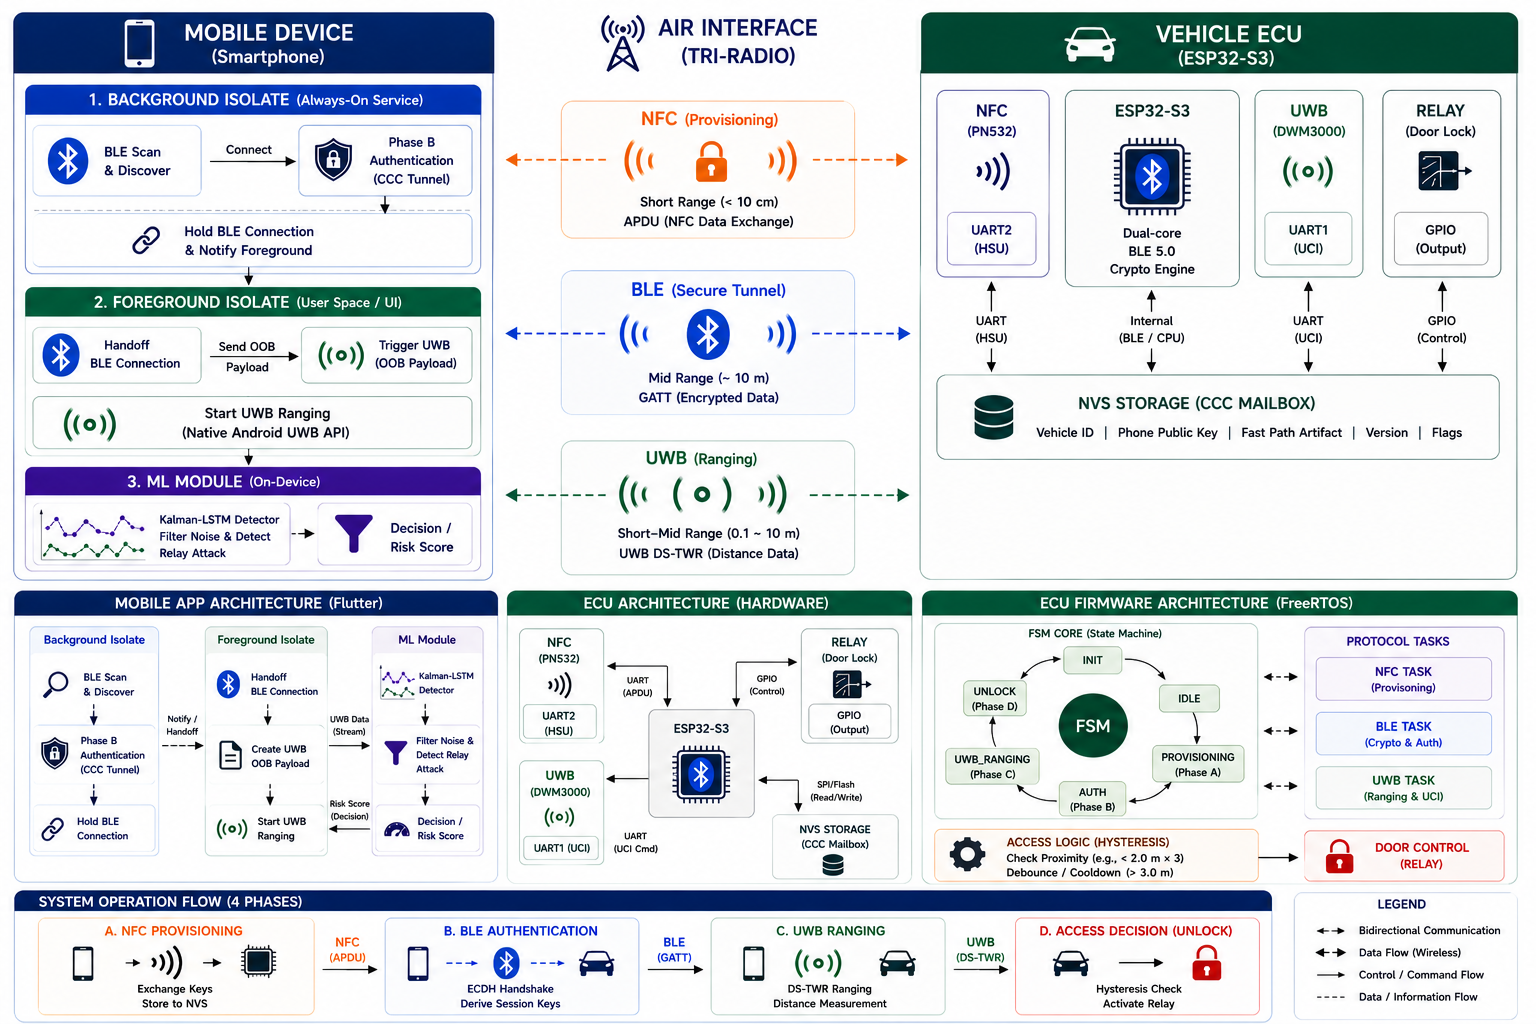
\includegraphics[width=1.0\textwidth]{image/section4/archi1.png} 
    \caption{Sơ đồ khối kiến trúc hệ thống Smart Car Access Tri-Radio}
    \label{fig:block_diagram}
\end{figure}

\subsection{Kiến trúc phần cứng ECU}

Hệ thống phần cứng trên xe được thiết kế module hóa nhằm tối ưu hóa hiệu năng giao tiếp đa kênh, bao gồm các thành phần:
\begin{itemize}
    \item \textbf{Core Microcontroller:} Vi điều khiển ESP32-S3 (Dual-core, tích hợp phần cứng mã hóa và BLE 5.0).
    \item \textbf{NFC Subsystem:} Sử dụng module PN532 phục vụ quá trình cấp quyền (Provisioning). Giao tiếp với ESP32 qua UART2 (RX=Pin 44, TX=Pin 43) sử dụng chế độ High Speed UART (HSU) ở tốc độ baud 115200.
    \item \textbf{UWB Subsystem:} Sử dụng vi mạch DWM3000 (được điều khiển bởi chip nRF52840 chạy UCI protocol firmware) để đo khoảng cách an toàn (Distance Bounding). Giao tiếp với ESP32 qua UART1 (RX=Pin 17, TX=Pin 18) thông qua giao thức UWB Command Interface (UCI).
    \item \textbf{Actuator (Cơ cấu chấp hành):} Module Relay khóa cửa, được điều khiển trực tiếp bởi chân GPIO (Digital Output) của ESP32.
\end{itemize}

\subsection{Kiến trúc phần mềm di động}

Để hiện thực hóa tính năng "Mở khóa không chạm" (Passive Keyless Entry) mà không làm tiêu hao tài nguyên pin, ứng dụng Flutter được chia thành hai không gian bộ nhớ (Isolates) tách biệt cùng với một module Trí tuệ nhân tạo:

\begin{itemize}
    \item \textbf{Background Isolate (Luồng chạy ngầm):} Quản lý bởi \texttt{PkeBackgroundService}. Nhiệm vụ của luồng này là liên tục quét (Scan) tín hiệu BLE dưới nền. Khi phát hiện xe, luồng tự động thiết lập kênh truyền an toàn và thực hiện Xác thực mật mã (Phase B). Điểm mấu chốt là sau khi xác thực, luồng này \textit{không ngắt kết nối} mà tiến hành "Giữ trạng thái" (Hold Connection) để bàn giao cho luồng Foreground.
    \item \textbf{Foreground Isolate (Luồng giao diện \& UWB Handoff):} Xử lý dịch vụ \texttt{UwbService} thông qua Native Android MethodChannel (\texttt{smartcar/uwb}). Kế thừa kết nối BLE từ Background, luồng này tạo gói tin OOB (Out-of-band Payload), gửi qua BLE Admin Characteristic (0x0005) cho ESP32, sau đó kích hoạt chip UWB trên điện thoại để bắt đầu phiên đo khoảng cách (Ranging).
    \item \textbf{Security \& ML Module:} Chứa thuật toán \textit{Kalman-LSTM Detector}. Tích hợp chức năng lọc nhiễu tọa độ UWB và phát hiện tấn công tiếp sóng (Relay Attack) dựa trên phân tích sự lạm phát khoảng cách trong chuỗi thời gian (Distance Inflation).
\end{itemize}

\subsection{Kiến trúc phần mềm vi điều khiển}

Firmware của ECU được thiết kế theo kiến trúc Event-Driven \& Multi-Tasking (Hướng sự kiện và Đa luồng) trên hệ điều hành thời gian thực FreeRTOS, đảm bảo xử lý đồng thời ba sóng vô tuyến mà không xảy ra nghẽn cổ chai.

\begin{itemize}
    \item \textbf{Core State Machine (Bộ não trung tâm - FSM Task):} Chạy trên một luồng riêng biệt, FSM quản lý toàn bộ vòng đời hệ thống (\texttt{INIT} $\rightarrow$ \texttt{IDLE} $\rightarrow$ \texttt{PROVISIONING} $\rightarrow$ \texttt{AUTH} $\rightarrow$ \texttt{UWB\_RANGING} $\rightarrow$ \texttt{UNLOCK}). FSM thu thập các sự kiện từ các task phần cứng và đưa ra quyết định chuyển trạng thái xuyên tầng (Cross-layer Security).
    \item \textbf{NFC Task:} Quản lý giao tiếp APDU với điện thoại trong Phase A, trao đổi khóa công khai và thiết lập các tham số Fast Path Artifact.
    \item \textbf{BLE Task (Crypto Engine):} Hoạt động trên nền thư viện NimBLE, cung cấp CCC Auth Service và Admin Service. Task này chịu trách nhiệm tính toán mật mã (mbedTLS): tạo cặp khóa ECDH Ephemeral, tính Shared Secret, băm HKDF-SHA256 sinh Session Keys, và xác thực chữ ký ECDSA.
    \item \textbf{UWB Task:} Quản lý giao thức UCI qua UART1 để cấu hình chip DWM3000, liên tục phân tích gói tin UCI Ranging Notification để trích xuất giá trị khoảng cách (\texttt{distanceM}) và trạng thái.
    \item \textbf{Door Unlock Module (Hysteresis Logic):} Đảm nhiệm quyết định mở cửa. Thuật toán yêu cầu khoảng cách đo được phải $\le 2.0$m trong 3 chu kỳ đo liên tiếp (Debounce) mới kích hoạt GPIO, và chỉ reset khi điện thoại ra khỏi vùng an toàn ($> 3.0$m).
    \item \textbf{CCC Mailbox:} Quản lý bộ nhớ Non-Volatile Storage (NVS) để lưu trữ tĩnh ID Xe, Public Key của điện thoại và các thông số cài đặt.
\end{itemize}

\begin{table}[H]
\centering
\begin{tabular}{|p{7.2cm}|p{7.2cm}|}
\hline
\textbf{Mobile App (Flutter Dual-Isolate)} & \textbf{Vehicle Controller (C/C++ FreeRTOS)} \\ \hline
\textbf{Background Isolate:} Quét BLE ngầm, tự động kết nối và chạy Phase B (Crypto) không cần mở màn hình. & \textbf{FSM Core:} Máy trạng thái hữu hạn kiểm soát tính nhất quán xuyên tầng (Cross-layer). \\ \hline
\textbf{Foreground Isolate:} Nhận Handoff, gọi API Native Android cấu hình chip UWB và gửi OOB. & \textbf{Tasks \& Protocol Layer:} NFC Task (APDU), BLE Task (GATT/Crypto), UWB Task (UCI Protocol). \\ \hline
\textbf{ML Layer:} Bộ lọc Kalman-LSTM phát hiện Relay Attack từ dữ liệu thô. & \textbf{Access Logic:} Thuật toán Hysteresis kết hợp dữ liệu Ranging để điều khiển GPIO Relay. \\ \hline
\end{tabular}
\caption{Tương quan kiến trúc phần mềm giữa Mobile App và ECU}
\label{tab:sw_arch_new}
\end{table}

\subsection{Luồng tương tác xuyên tầng}

Để đảm bảo an ninh vật lý và logic, hệ thống thực thi chuỗi giao dịch xuyên qua ba giao thức độc lập theo trình tự nghiêm ngặt sau:

\begin{enumerate}
    \item \textbf{Phase A: Cấp phép vật lý (Physical Root-of-Trust) - NFC} \\
    Đầu tiên người dùng thêm thông tin xe bằng cách sử dụng app quét thẻ master card, Sau đó người dùng chạm điện thoại vào NFC Reader. \texttt{NFCTask} nhận diện thẻ HCE, chuyển FSM sang trạng thái \texttt{PROVISIONING}. Hai thiết bị trao đổi Public Keys và lưu vào \texttt{CCCMailbox}.
    
    \item \textbf{Phase B: Xác thực bảo mật (Cryptographic Session Binding) - BLE} \\
    Khi người dùng tiến vào vùng Welcome Zone ($\sim 10$m), \texttt{PkeBackgroundService} tự động kết nối BLE. ESP32 chuyển FSM sang \texttt{AUTH}. Hai bên sinh khóa tạm thời ECDH, ký xác nhận bằng khóa NFC đã lưu, dẫn xuất ra các Khóa phiên (Session Keys).
    
    \item \textbf{Phase C: Xác thực khoảng cách (Physical Distance Bounding) - UWB} \\
    Sau khi Phase B thành công, điện thoại gửi cấu hình UWB (OOB Payload) qua đường hầm BLE. ESP32 đẩy OOB sang \texttt{UWBTask} để bật vi mạch DWM3000. Giao thức DS-TWR (Double-Sided Two-Way Ranging) hoạt động, liên tục trả về các thông số khoảng cách ($1.5$m, $1.3$m, $0.8$m...).
    
    \item \textbf{Phase D: Quyết định mở cửa (Conjunctive Access Decision)} \\
    Dữ liệu khoảng cách từ Phase C được đẩy vào mạng lọc Hysteresis. Nếu hệ thống ghi nhận 3 lần liên tiếp khoảng cách $< 2.0$m \textbf{VÀ} FSM đang ở trạng thái \texttt{AUTH\_SECURE\_CHANNEL\_READY} (Đã xác thực BLE), ESP32 mới cấp điện cho GPIO kích hoạt Relay mở cửa.
\end{enumerate}







%------------------------------------------------------------------------------------







\section{Lựa chọn nền tảng phần cứng}

Việc lựa chọn phần cứng đóng vai trò then chốt trong việc hiện thực hóa các giao thức bảo mật phức tạp và xử lý đồng thời đa vô tuyến trong thời gian thực.

\subsection{Yêu cầu về phần cứng trung tâm}
Bộ điều khiển trung tâm cần đáp ứng các tiêu chí:
\begin{itemize}
    \item Hỗ trợ cấu hình nhiều giao tiếp ngoại vi độc lập (UART/SPI) để kết nối NFC và UWB mà không nghẽn cổ chai.
    \item Có khả năng xử lý các thuật toán mã hóa (ECDH, ECDSA, AES), ưu tiên có bộ tăng tốc phần cứng (Hardware Accelerator).
    \item Có bộ nhớ lưu trữ không bay hơi (NVS) và đủ dung lượng RAM cho RTOS đa luồng.
\end{itemize}

\subsection{Phân tích và lựa chọn: Automotive ECU vs. ESP32-S3}

\subsubsection{Target Platform: Automotive ECU}
Các ECU tiêu chuẩn công nghiệp (như Bosch EDC17, Continental BCM) sử dụng kiến trúc ARM Cortex-M4/M7, tuân thủ chuẩn AUTOSAR và ISO 26262. Tuy nhiên, rào cản lớn nhất đối với nghiên cứu là chi phí đắt đỏ (\$500-\$2000/unit) và độ phức tạp cực kỳ cao trong việc tiếp cận công cụ phát triển (Vector CANoe).

\subsubsection{Development Platform: ESP32-S3}
Nhóm quyết định sử dụng ESP32-S3 làm nền tảng phát triển Proof-of-Concept (PoC) dựa trên các lợi thế kỹ thuật chuyên sâu \cite{esp32s3}:

\textbf{A. Thông số kỹ thuật ESP32-S3:}
\begin{itemize}
    \item \textbf{MCU:} Xtensa LX7 dual-core hoạt động ở xung nhịp 240 MHz, cung cấp năng lực xử lý vượt trội.
    \item \textbf{Crypto Engine:} Tích hợp bộ tăng tốc phần cứng cho AES, SHA, RSA, RNG.
    \item \textbf{Wireless:} Tích hợp sẵn Wi-Fi và BLE 5.0 Native.
    \item \textbf{Peripherals:} Hỗ trợ ma trận phần cứng linh hoạt, cho phép cấu hình 2 luồng UART độc lập (UART1 cho DWM3000, UART2 cho PN532) không xung đột.
\end{itemize}

\textbf{B. So sánh kỹ thuật chi tiết:}

\begin{table}[H]
\centering
\begin{tabularx}{\textwidth}{|l|X|X|X|}
\hline
\textbf{Tiêu chí} & \textbf{Automotive ECU} & \textbf{ESP32-S3} & \textbf{Đánh giá} \\ \hline
Processing Power & ARM M4/M7 & Xtensa LX7 @240MHz & Tương đương \\ \hline
Crypto HW & Có & Có (AES, SHA Accel) & Đạt yêu cầu \\ \hline
Kết nối nội bộ & Multi-bus & Ma trận linh hoạt (Multi-UART) & Rất phù hợp cho UWB/NFC \\ \hline
Chi phí & \$500 - \$2000 & $\approx$ \$5 & ESP32 tối ưu \\ \hline
Safety Cert & ISO 26262 & Không có & Hạn chế của ESP32 \\ \hline
Development & Phức tạp (AUTOSAR) & Linh hoạt (FreeRTOS/C++) & ESP32 dễ tiếp cận \\ \hline
\end{tabularx}
\caption{So sánh Automotive ECU và ESP32-S3}
\end{table}

\textbf{C. Kết quả Benchmark hiệu năng Crypto:}
Để chứng minh khả năng đáp ứng thời gian thực (đặc biệt khi kết hợp luồng đo UWB), nhóm đã thực hiện đo đạc trên ESP32-S3 (sử dụng thư viện mbedTLS):
\begin{itemize}
    \item ECDH key exchange (P-256): \textbf{85ms} (Mục tiêu $< 100$ms).
    \item ECDSA verify (P-256): \textbf{95ms}.
    \item AES-128-GCM encrypt (1KB): \textbf{12ms}.
    \item \textbf{Tổng thời gian luồng xác thực BLE:} \textbf{< 400ms} (Dư dả thời gian cấp quyền bật UWB).
\end{itemize}

\textbf{Kết luận:} ESP32-S3 hoàn toàn đáp ứng được các yêu cầu khắt khe về thời gian phản hồi, khả năng quản lý đa luồng FreeRTOS cho giao thức Tri-Radio, đồng thời tối ưu hóa thời gian và chi phí phát triển R\&D.

\subsection{Kiến trúc chuyển đổi}
Để đảm bảo tính khả thi khi chuyển đổi từ ESP32 sang ECU thực tế trong tương lai, hệ thống phần mềm được thiết kế theo kiến trúc phân lớp (Layered Architecture):

\begin{itemize}
    \item \textbf{Application Layer:} Chứa logic FSM, Access Control. Tầng này độc lập với phần cứng.
    \item \textbf{Protocol Layer:} Xử lý APDU, BLE GATT, UCI Parser. Tuân thủ tiêu chuẩn quốc tế.
    \item \textbf{Hardware Abstraction Layer (HAL):} Tầng trung gian quản lý UART/GPIO. Hiện tại HAL map vào ESP-IDF, trong tương lai có thể map vào AUTOSAR BSW \cite{iso26262}.
\end{itemize}

Việc tách biệt này giúp tái sử dụng phần lớn mã nguồn C/C++ khi thay đổi phần cứng vi điều khiển.





%------------------------------------------------------------------------------------





\section{Thiết kế giao thức bảo mật}

Kiến trúc bảo mật của hệ thống được thiết kế phân lớp, tuân thủ nghiêm ngặt chuẩn CCC Digital Key Release 3.0 nhằm triệt tiêu các rủi ro tấn công tiếp sóng và giả mạo thiết bị. Quá trình từ khi người dùng chưa có quyền đến khi mở cửa xe thành công được chia thành 4 giai đoạn (Phases) với trách nhiệm bảo mật chuyên biệt.

\subsection{Phase A - Giai đoạn Cấp quyền vật lý}
Phase A thiết lập mối quan hệ tin cậy nền tảng (Root-of-Trust) giữa điện thoại thông minh và ECU của xe thông qua kênh giao tiếp vật lý tầm ngắn NFC (Out-of-Band). Sự giới hạn về khoảng cách của NFC ($< 10$cm) chính là lớp khiên vật lý chống lại các hành vi nghe lén.

\leavevmode
\begin{figure}[htbp]
    \centering
    % Sinh viên lưu ý cập nhật ảnh Sơ đồ kiến trúc mới có đủ NFC, BLE, UWB và luồng Dual-Isolate nhé
    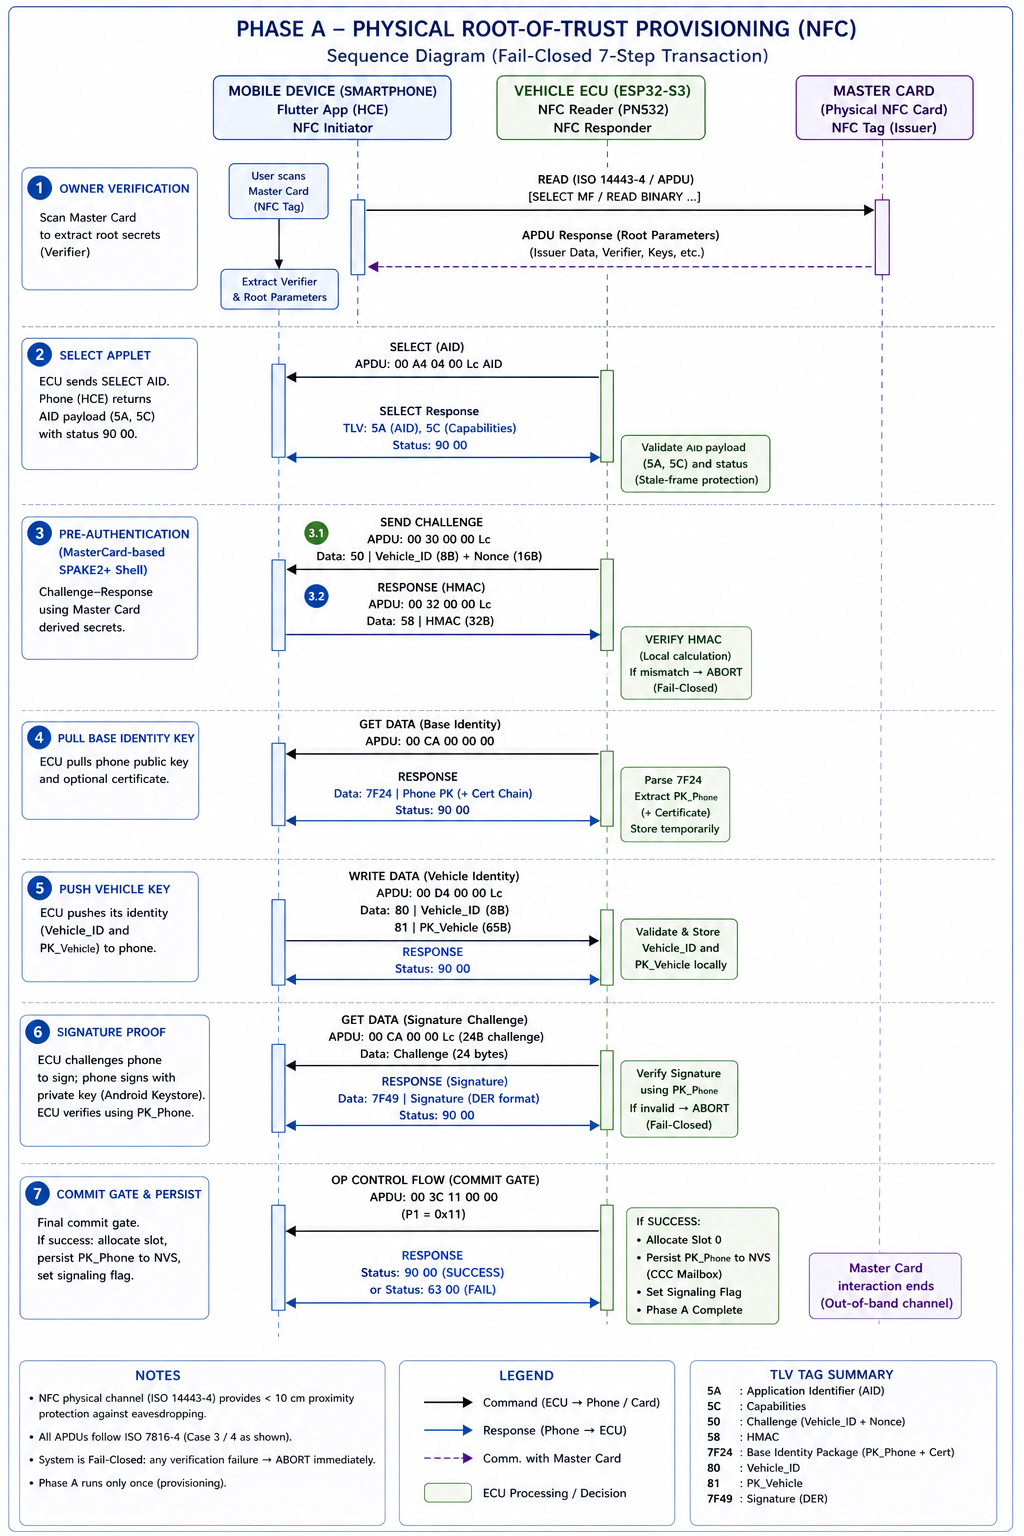
\includegraphics[width=0.9\textwidth]{image/section4/phaseAnew.png} 
    \caption{Sơ đồ Sequence Phase A}
    \label{fig:phaseA}
\end{figure}

Nhằm tăng cường độ tin cậy và chống lại các khung dữ liệu cũ/trễ (Stale-frame), hệ thống không sử dụng luồng cấp quyền đơn giản mà áp dụng một quy trình giao dịch \textit{Fail-Closed} nghiêm ngặt gồm 7 bước:

\begin{enumerate}
    \item \textbf{Xác thực quyền sở hữu qua thẻ Master Card (Owner Verification):} 
    Trước khi tương tác với xe, người dùng phải sử dụng điện thoại thông minh để quét thẻ NFC vật lý Master Card (thẻ gốc do nhà sản xuất cấp) thông qua đầu đọc NFC tích hợp trên điện thoại. Bước này giúp ứng dụng trích xuất các tham số mật mã nền tảng (Verifier) nhằm chứng minh người dùng là chủ sở hữu hợp pháp của phương tiện trước khi bắt đầu quy trình cấp quyền.

    \item \textbf{Lựa chọn Applet (SELECT AID):} 
    Người dùng đưa điện thoại (lúc này đang kích hoạt chế độ mô phỏng thẻ HCE) chạm vào đầu đọc NFC (PN532) trên xe. ECU lập tức gửi lệnh \texttt{SELECT AID} chuẩn ISO 7816-4. Ứng dụng HCE trên điện thoại phản hồi các thẻ dữ liệu (payload tags \texttt{5A, 5C}) kèm mã trạng thái \texttt{90 00}. ECU thực hiện xác thực chéo nội dung payload nhằm loại bỏ hoàn toàn các khung dữ liệu rác (Stale-frame protection).

    \item \textbf{Xác thực sơ bộ (MasterCard-based SPAKE2+ Shell):} 
    Hệ thống áp dụng cơ chế xác thực mô phỏng chuẩn MasterCard để xác minh dữ liệu quét được từ bước 1. ESP32 tạo một thông điệp thử thách (Challenge) gồm định danh xe (\texttt{Vehicle\_ID} - 8 bytes) và chuỗi ngẫu nhiên (Nonce - 16 bytes). 
    \begin{itemize}
        \item ECU gửi Challenge qua lệnh APDU \texttt{0x30} (được bọc trong thẻ TLV \texttt{0x50}).
        \item Điện thoại sử dụng thông tin từ thẻ Master Card để tính toán, sau đó phản hồi lệnh yêu cầu xác thực \texttt{0x32} bằng mã băm HMAC (thẻ TLV \texttt{0x58}). 
        \item ESP32 tính toán HMAC cục bộ và đối chiếu. Nếu dữ liệu không khớp hoàn toàn, giao dịch lập tức bị hủy.
    \end{itemize}

    \item \textbf{Rút khóa định danh cơ sở (Base Key Exchange Pull):} 
    ECU gửi lệnh \texttt{GET DATA} (INS \texttt{0xCA}, \texttt{Lc=0}). Điện thoại trả về gói định danh cơ sở (bọc bởi tag \texttt{7F24}). ESP32 tiến hành phân tách gói tin để thu thập Khóa công khai của điện thoại ($PK_{Phone}$) và chuỗi chứng chỉ tùy chọn.

    \item \textbf{Đẩy khóa định danh xe (Vehicle Key Exchange Push):} 
    Để thiết lập ràng buộc hai chiều, ECU chủ động gửi lệnh \texttt{WRITE DATA} (INS \texttt{0xD4}) đẩy dữ liệu sang điện thoại. Các tham số bao gồm \texttt{Vehicle\_ID} (TLV \texttt{0x80}) và Khóa công khai của xe $PK_{Vehicle}$ (TLV \texttt{0x81}). Ứng dụng điện thoại sẽ xác thực và lưu trữ các tham số này cục bộ.

    \item \textbf{Chứng minh bằng chữ ký (Signature Proof):} 
    ECU gửi một lệnh \texttt{GET DATA} (INS \texttt{0xCA}) thứ hai mang theo một Challenge dài 24 bytes vào vùng dữ liệu APDU. Điện thoại bắt buộc phải ký chuỗi này bằng Private Key được bảo vệ sâu trong Android Keystore và trả về chữ ký định dạng DER. ESP32 sử dụng $PK_{Phone}$ vừa nhận được ở bước 4 để xác thực chữ ký này.

    \item \textbf{Cổng cam kết và Lưu trữ (Commit Gate \& Persist):} 
    Nếu chữ ký hoàn toàn hợp lệ, ECU tiến hành gửi lệnh \texttt{OP CONTROL FLOW} (INS \texttt{0x3C}, tham số \texttt{P1=0x11}) làm "Cổng cam kết" cho giao dịch. Chỉ khi bước chốt chặn này báo thành công, ESP32 mới cấp phát Slot 0, lưu trữ vĩnh viễn $PK_{Phone}$ vào bộ nhớ bảo mật NVS (CCC Mailbox) và bật cờ tín hiệu (Signaling flag). Phase A chính thức kết thúc.
\end{enumerate}

Phase A chỉ diễn ra một lần duy nhất. Giai đoạn này không thực hiện mở khóa xe mà đóng vai trò gieo mầm (Seeding) các khóa định danh dài hạn cho các pha xác thực vô tuyến tiếp theo.

\subsection{Phase B - Xác thực bảo mật kênh truyền}
Giai đoạn B thiết lập một đường hầm bảo mật (Secure Tunnel) tầm xa giữa điện thoại và xe qua sóng Bluetooth Low Energy (BLE). Mục tiêu của Phase B \textbf{không phải là mở cửa xe}, mà là để chứng minh quyền sở hữu khóa (Proof of Ownership) và sinh ra các khóa phiên (Session Keys).

\leavevmode
\begin{figure}[htbp]
    \centering
    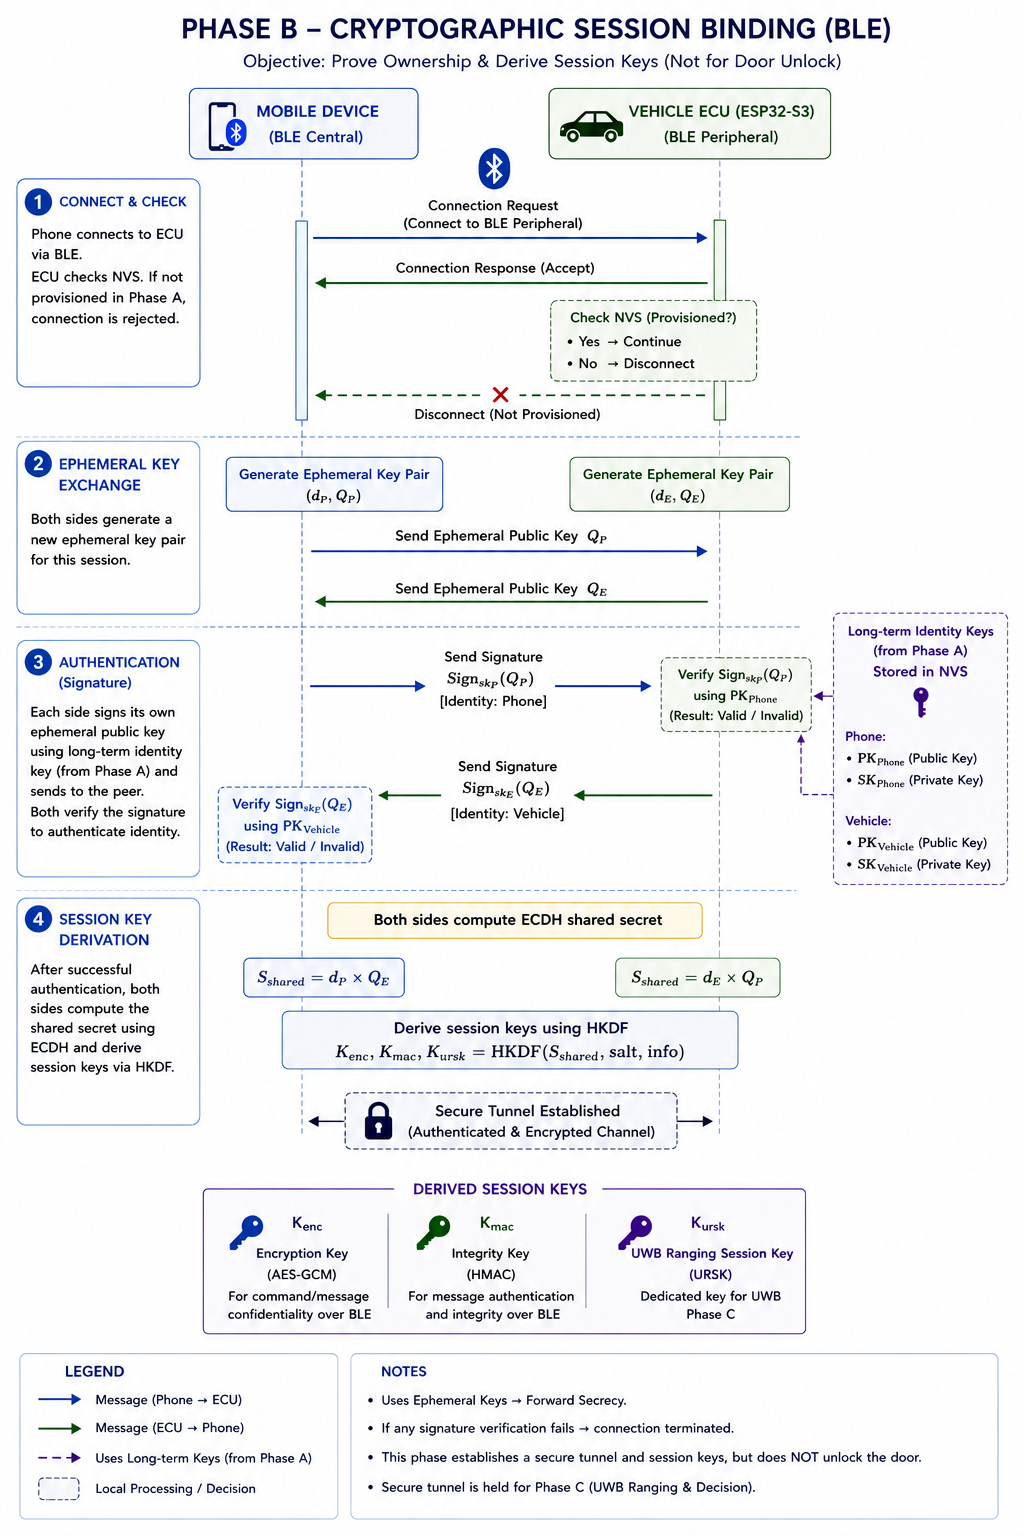
\includegraphics[width=0.9\textwidth]{image/section4/phaseBnew.png} 
    \caption{Sơ đồ Sequence Phase B}
    \label{fig:phaseB}
\end{figure}

\textbf{Quy trình bắt tay 3 bước (3-Way Handshake) dựa trên ECDH:}
\begin{enumerate}
    \item \textbf{Kết nối và Kiểm tra:} Điện thoại (BLE Central) tiến vào vùng phủ sóng và kết nối với ESP32 (BLE Peripheral). ESP32 kiểm tra trạng thái NVS, nếu chưa được Provisioning ở Phase A, kết nối lập tức bị ngắt.
    \item \textbf{Trao đổi khóa tạm thời (Ephemeral Key Exchange):} Cả hai thiết bị sinh một cặp khóa đường cong Elliptic tạm thời (Ephemeral Keys) hoàn toàn mới cho phiên kết nối hiện tại.
    \item \textbf{Xác thực danh tính (Authentication):} Mỗi bên dùng Khóa định danh dài hạn (đã lưu ở Phase A) để ký lên Khóa tạm thời của mình rồi gửi cho đối phương. Quá trình này giúp hai bên xác minh chắc chắn danh tính của nhau.
    \item \textbf{Dẫn xuất khóa phiên (Session Key Derivation):} Sau khi xác thực chữ ký, hai bên dùng thuật toán ECDH để tính ra bí mật chung ($S_{shared}$). Từ đó, sử dụng hàm KDF (Key Derivation Function) \cite{rfc5869} để sinh ra các khóa dùng một lần:
\end{enumerate}

\begin{equation}
    K_{enc}, K_{mac}, K_{ursk} = \text{HKDF}(S_{shared}, \text{salt}, \text{info})
\end{equation}

Trong đó:
\begin{itemize}
    \item $K_{enc}, K_{mac}$: Khóa dùng để mã hóa (AES-GCM) và xác thực toàn vẹn (HMAC) các thông điệp lệnh qua BLE \cite{fips197}.
    \item $K_{ursk}$: Khóa Ranging Session Key dành riêng cho giao thức UWB ở Phase C \cite{neirynck2016overview}.
\end{itemize}

Việc sử dụng Ephemeral Keys đảm bảo tính \textbf{Bảo mật chuyển tiếp (Forward Secrecy)}: Dù kẻ gian có giải mã được khóa của một phiên kết nối cũ, chúng cũng không thể can thiệp vào các phiên kết nối hiện tại hay tương lai.

\subsection{Phase C - Xác thực khoảng cách an toàn với UWB}
Khác với các hệ thống Smart Key truyền thống dùng RSSI của Bluetooth để đo khoảng cách (vốn dễ bị khuyếch đại bởi các bộ lặp Relay), hệ thống sử dụng công nghệ UWB (Ultra-Wideband) làm thước đo vật lý chính xác tuyệt đối.

\leavevmode
\begin{figure}[htbp]
    \centering
    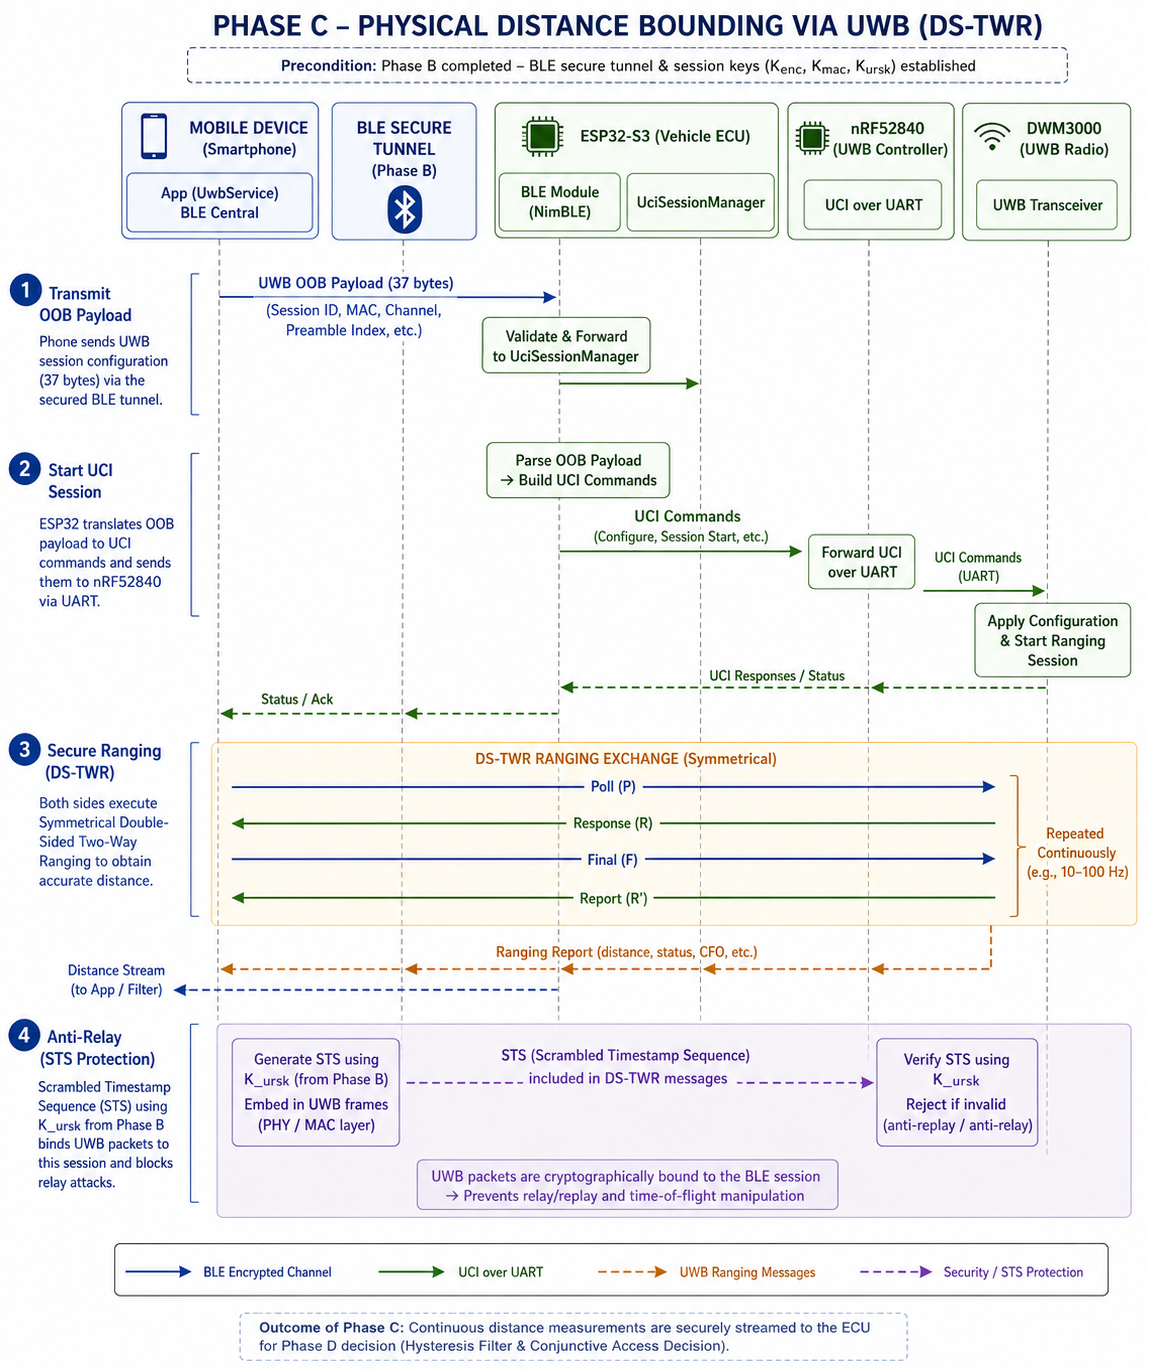
\includegraphics[width=0.9\textwidth]{image/section4/phaseCnew.png} 
    \caption{Sơ đồ Sequence Phase C}
    \label{fig:phaseC}
\end{figure}

\begin{enumerate}
    \item \textbf{Truyền OOB Payload:} Thông qua đường hầm BLE đã được bảo mật ở Phase B, điện thoại gửi một gói \textit{Out-Of-Band (OOB) Payload} (37 bytes) chứa cấu hình phiên UWB (Session ID, MAC Address, Channel, Preamble Index) đến ESP32.
    \item \textbf{Khởi động phiên UCI:} ESP32 (lớp \texttt{UciSessionManager}) dịch OOB Payload thành các lệnh UWB Command Interface (UCI) và đẩy xuống vi mạch nRF52840 gắn shield DWM3000 thông qua giao tiếp UART1. Từ đó Ranging session sẽ được thiết lập.
    \item \textbf{Đo khoảng cách (Secure Ranging):} Vi mạch UWB hai bên bắt đầu phát xung. Giao thức \textbf{Symmetrical Double-Sided Two-Way Ranging (DS-TWR)} được sử dụng nhằm triệt tiêu hoàn toàn sai số trôi đồng hồ (Clock drift) giữa điện thoại và xe.
    \item \textbf{Chống Relay Attack:} Để ngăn chặn kẻ gian thu phát lại tín hiệu xung UWB, một chuỗi dấu thời gian bị xáo trộn (Scrambled Timestamp Sequence - STS) được áp dụng vào tầng vật lý (MAC layer) \cite{ccc_digikey3, nxp_ncj29d5, neirynck2016overview}. STS được mã hóa bằng chính khóa $K_{ursk}$ đã sinh ra từ Phase B \cite{neirynck2016overview}. Nhờ đó, gói tin UWB bị ràng buộc chặt chẽ với phiên BLE, triệt tiêu mọi khả năng chèn ép hoặc làm giả thời gian bay (Time-of-Flight).
\end{enumerate}

\subsection{Phase D - Quyết định truy cập thông minh dựa trên học sâu}

Đây là giai đoạn thực thi cuối cùng và quan trọng nhất của hệ thống. Việc kích hoạt rơ-le mở cửa (Door Unlock Actuator) không còn phụ thuộc vào các ngưỡng khoảng cách tĩnh đơn lẻ, mà là kết quả của sự \textbf{quyết định kết hợp} giữa trạng thái giao thức, dữ liệu vật lý thời gian thực và kết quả suy luận từ mô hình học sâu chuỗi thời gian.

\leavevmode
\begin{figure}[htbp]
    \centering
    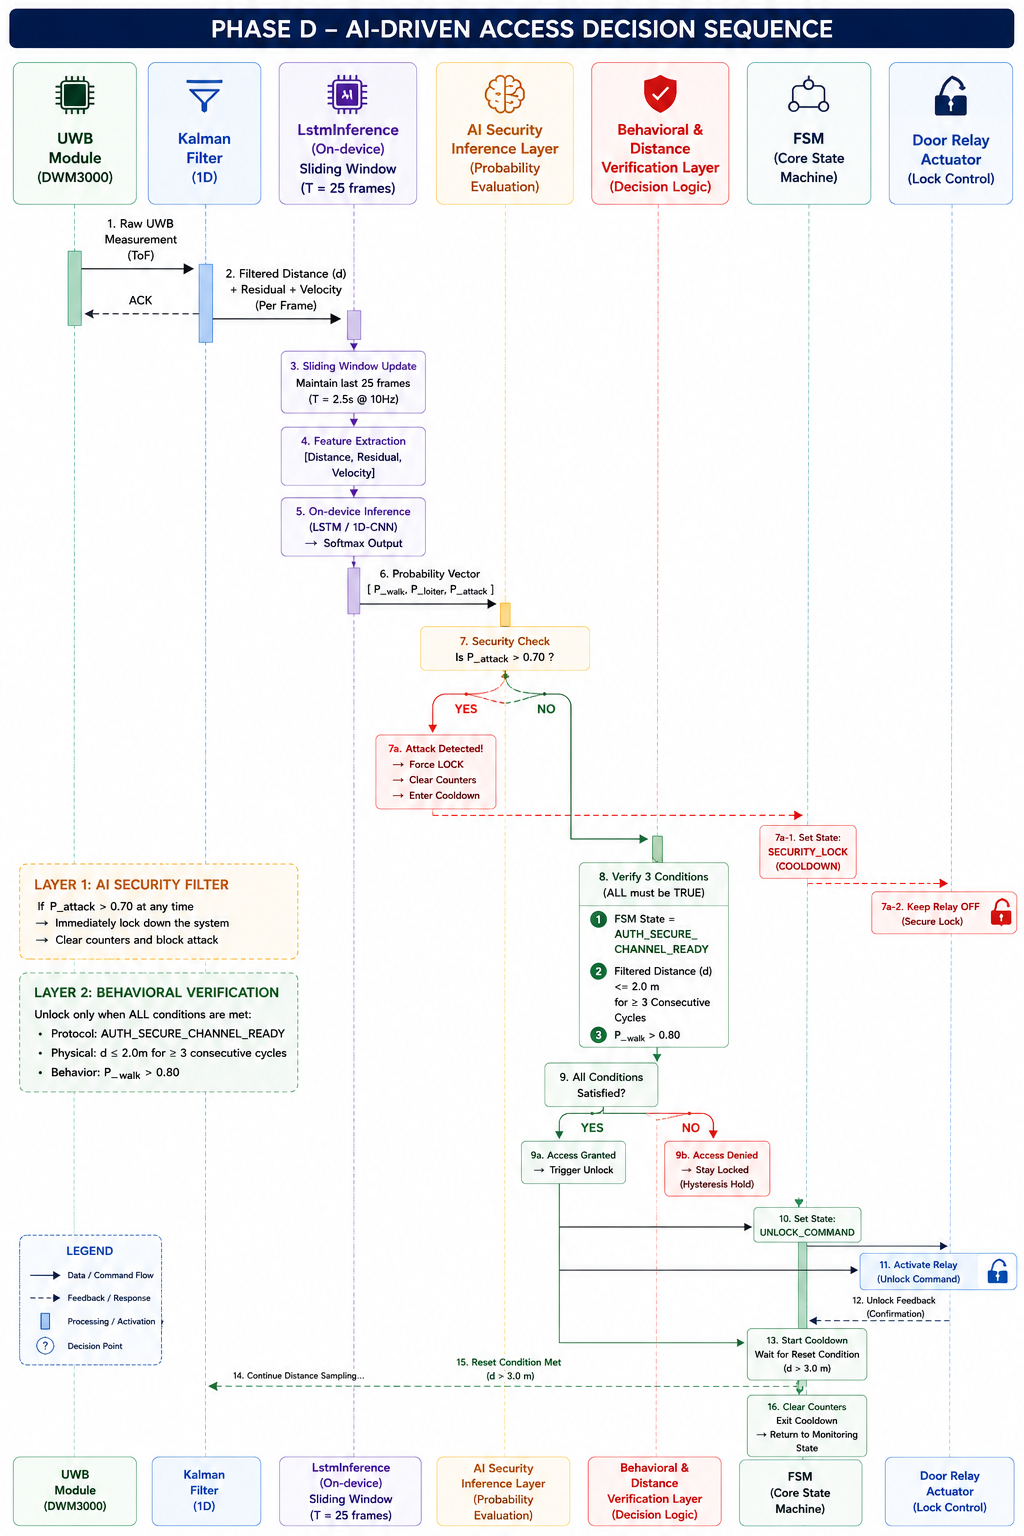
\includegraphics[width=0.8\textwidth]{image/section4/phaseDnew2.png} 
    \caption{Sơ đồ Sequence Phase D tích hợp suy luận AI}
    \label{fig:phaseD}
\end{figure}

Dữ liệu UWB sau khi đi qua bộ lọc Kalman sẽ được đưa vào module \texttt{LstmInference}. Tại đây, một cửa sổ trượt (Sliding Window) lưu trữ $25$ khung hình gần nhất sẽ thực hiện tính toán đặc trưng và suy luận ngay trên vi điều khiển (On-device Inference). Quy trình ra quyết định được thực hiện qua hai lớp bảo mật:

\begin{enumerate}
    \item \textbf{Lớp lọc an ninh AI (Security Inference Layer):}
    Hệ thống liên tục đánh giá vector xác suất từ mô hình AI bao gồm $P_{walk}$ (Tiếp cận), $P_{loiter}$ (Lảng vảng) và $P_{attack}$ (Tấn công tiếp sóng). 
    \begin{itemize}
        \item Nếu ghi nhận xác suất tấn công $P_{attack} > 0.70$, hệ thống lập tức cưỡng bức trạng thái khóa an toàn, ngăn chặn hoàn toàn mọi nỗ lực xâm nhập bằng thiết bị tiếp sóng ngay cả khi khoảng cách vật lý thỏa mãn điều kiện.
    \end{itemize}

    \item \textbf{Lớp xác thực hành vi và khoảng cách (Behavioral Verification Layer):}
    Rơ-le cửa chỉ được phép kích hoạt \textbf{NẾU VÀ CHỈ NẾU} thỏa mãn đồng thời ba điều kiện sau:
    \begin{itemize}
        \item \textbf{Giao thức:} FSM đang ở trạng thái \texttt{AUTH\_SECURE\_CHANNEL\_READY} (Đã xác thực BLE thành công).
        \item \textbf{Vật lý:} Khoảng cách UWB đã lọc ($d$) nằm trong ngưỡng tiệm cận ($\le 2.0$ mét) trong ít nhất \textbf{3 chu kỳ đo liên tiếp}.
        \item \textbf{Hành vi:} Mô hình AI xác nhận ý định người dùng với độ tin cậy $P_{walk} > 0.80$. Điều này giúp loại bỏ hoàn toàn các trường hợp người dùng vô tình đi ngang qua vùng nhận diện hoặc dừng lại ở ranh giới 2m nhưng không có ý định vào xe.
    \end{itemize}
\end{enumerate}

\paragraph*{Điều kiện phục hồi (Cooldown):} 
Sau khi thực hiện lệnh mở cửa, hệ thống sẽ đi vào trạng thái cooldown. Cơ chế Reset chỉ được kích hoạt khi người dùng rời khỏi vùng thiết lập lại (Reset Zone, ví dụ $d > 3.0$ mét), đảm bảo tính ổn định và tránh việc rơ-le hoạt động thừa thãi.

Sự kết hợp giữa lý thuyết điều khiển truyền thống (Hysteresis) và trí tuệ nhân tạo (TinyML) giúp hệ thống Smart Car Access đạt được độ tin cậy vượt trội, mang lại trải nghiệm mở khóa thụ động (PKE) mượt mà nhưng vẫn đảm bảo tính an toàn tuyệt đối trước các hình thức tấn công công nghệ cao hiện nay.

% =======================================================================


\subsection{Cơ chế đánh giá hành vi dựa trên mô hình chuỗi thời gian}

Trong các hệ thống PKE (Passive Keyless Entry) truyền thống, việc ra quyết định mở cửa chỉ dựa trên một ngưỡng khoảng cách tĩnh (ví dụ: $d \le 2.0$m). Tuy nhiên, phương pháp này tồn tại hai lỗ hổng lớn: không thể nhận diện được các bước nhảy vọt của khoảng cách do tấn công tiếp sóng (Relay Attack), và không phân biệt được người dùng đang chủ đích tiến vào xe hay chỉ đang đứng nói chuyện/lảng vảng gần xe (Loitering).

Để giải quyết triệt để bài toán này, kiến trúc hệ thống đã tích hợp thêm một lớp đánh giá hành vi sử dụng mô hình học sâu (Deep Learning) xử lý chuỗi thời gian, vận hành song song với bộ đệm Hysteresis. Cơ chế đánh giá được thực hiện qua các bước sau:

\paragraph*{Cửa sổ thời gian và Trích xuất đặc trưng: }
Thay vì đánh giá từng khung hình rời rạc, hệ thống duy trì một cửa sổ trượt (Sliding Window) có kích thước $T = 25$ khung hình (tương đương với chu kỳ $2.5$ giây ở tần số lấy mẫu 10Hz). Tại mỗi khung hình, bộ tiền xử lý sẽ trích xuất 3 đặc trưng vật lý quan trọng:
\begin{itemize}
    \item \textbf{Khoảng cách đã lọc (Filtered Distance):} Dữ liệu quỹ đạo đi bộ sau khi đi qua bộ lọc Kalman 1D.
    \item \textbf{Thặng dư Kalman (Residual):} Sự chênh lệch giữa phép đo UWB thô và giá trị dự báo của bộ lọc. Đây là đặc trưng tối quan trọng, vì các thiết bị Relay Attack khi khuếch đại tín hiệu sẽ tạo ra độ trễ phần cứng, dẫn đến sự sai lệch đột biến về Thời gian bay (ToF), làm giá trị Residual tăng vọt.
    \item \textbf{Vận tốc tức thời (Velocity):} Đạo hàm bậc 1 của khoảng cách theo thời gian. Đặc trưng này giúp mô hình nhận biết hướng di chuyển (tiến lại gần, lùi ra xa) và trạng thái dừng lại.
\end{itemize}

\paragraph*{Phân loại xác suất hành vi: }
Ma trận dữ liệu đầu vào có kích thước $(25 \times 3)$ sẽ được chuẩn hóa (Z-score Normalization) dựa trên các tham số cấu hình tĩnh (Mean, Scale) từ tập dữ liệu huấn luyện trước khi đưa vào mạng nơ-ron (LSTM/1D-CNN) trên vi điều khiển.
Mô hình sẽ tính toán và xuất ra phân bố xác suất (Softmax) cho 3 kịch bản hành vi:
\begin{itemize}
    \item $P(\text{Walk})$: Xác suất người dùng đang chủ đích bước tới xe.
    \item $P(\text{Loiter})$: Xác suất người dùng đang lảng vảng, đi ngang qua hoặc dừng lại ở ranh giới ngoài mà không có ý định mở cửa.
    \item $P(\text{Attack})$: Xác suất tín hiệu đang bị thao túng bởi trạm lặp (Relay Station).
\end{itemize}

\paragraph*{Tích hợp AI vào Logic điều khiển cơ học: }
Xác suất đầu ra từ mô hình AI không thay thế hoàn toàn cơ chế Hysteresis cơ học mà đóng vai trò như một màng lọc bảo mật cấp cao (High-level Security Gate). Quyết định điều khiển rơ-le mở cửa được thiết kế dựa trên logic kết hợp như sau:
\begin{itemize}
    \item \textbf{Ưu tiên an ninh tuyệt đối:} Nếu bất kỳ thời điểm nào hệ thống ghi nhận $P(\text{Attack}) > 0.70$, hệ thống lập tức từ chối mở cửa và làm trống bộ đệm (Reset counter), vô hiệu hóa hoàn toàn cuộc tấn công.
    \item \textbf{Xử lý nhiễu biên (Edge-case Handling):} Khi người dùng bước vào vùng $< 2.0$m nhưng đột ngột khựng lại hoặc quay lưng bước đi, vận tốc sẽ thay đổi nhanh chóng làm $P(\text{Loiter})$ tăng cao và $P(\text{Walk})$ giảm sút. Rơ-le sẽ không kích hoạt, triệt tiêu hiện tượng mở cửa sai (False Positive).
    \item \textbf{Kích hoạt mở cửa an toàn:} Rơ-le chỉ nhả chốt khi thỏa mãn đồng thời hai điều kiện vật lý và động học: Người dùng đã nằm trong vùng tiệm cận ($d \le 2.0$m) trong 3 chu kỳ đo liên tiếp và AI xác nhận độ tin cậy của hành động tiếp cận ($P(\text{Walk}) > 0.80$).
\end{itemize}

Kết hợp này tạo ra một kiến trúc "Phòng thủ chiều sâu" (Defense-in-depth), nơi thuật toán truyền thống đảm bảo tính an toàn cơ học, còn AI cung cấp lớp bảo mật chống giả mạo vật lý.




%------------------------------------------------------------------------------------








\section{Thiết kế kiến trúc máy trạng thái hữu hạn - FSM}

Trong hệ thống Smart Car Access, máy trạng thái hữu hạn (Finite State Machine - FSM) được sử dụng làm trung tâm điều phối xuyên tầng (Cross-layer Coordinator) để quản lý toàn bộ vòng đời hoạt động của hệ thống. Dựa trên kiến trúc Tri-Radio của chuẩn CCC, FSM phải đồng bộ hóa trạng thái giữa ba tiến trình phần cứng độc lập: NFC (Provisioning - Phase A), BLE (Authentication - Phase B) và UWB (Secure Ranging - Phase C/D) \cite{fsm_book}.

FSM cho phép hệ thống vận hành theo nguyên tắc \textit{Fail-Closed}, có thể kiểm chứng toán học, ngăn chặn các rủi ro bảo mật như tấn công hạ cấp (Downgrade Attack) bằng cách đảm bảo hệ thống không bao giờ bỏ qua các trạng thái xác thực trung gian.

\leavevmode
\begin{figure}[htbp]
    \centering
    % Hãy chèn ảnh FSM Flowchart cập nhật có đủ luồng UWB vào đây
    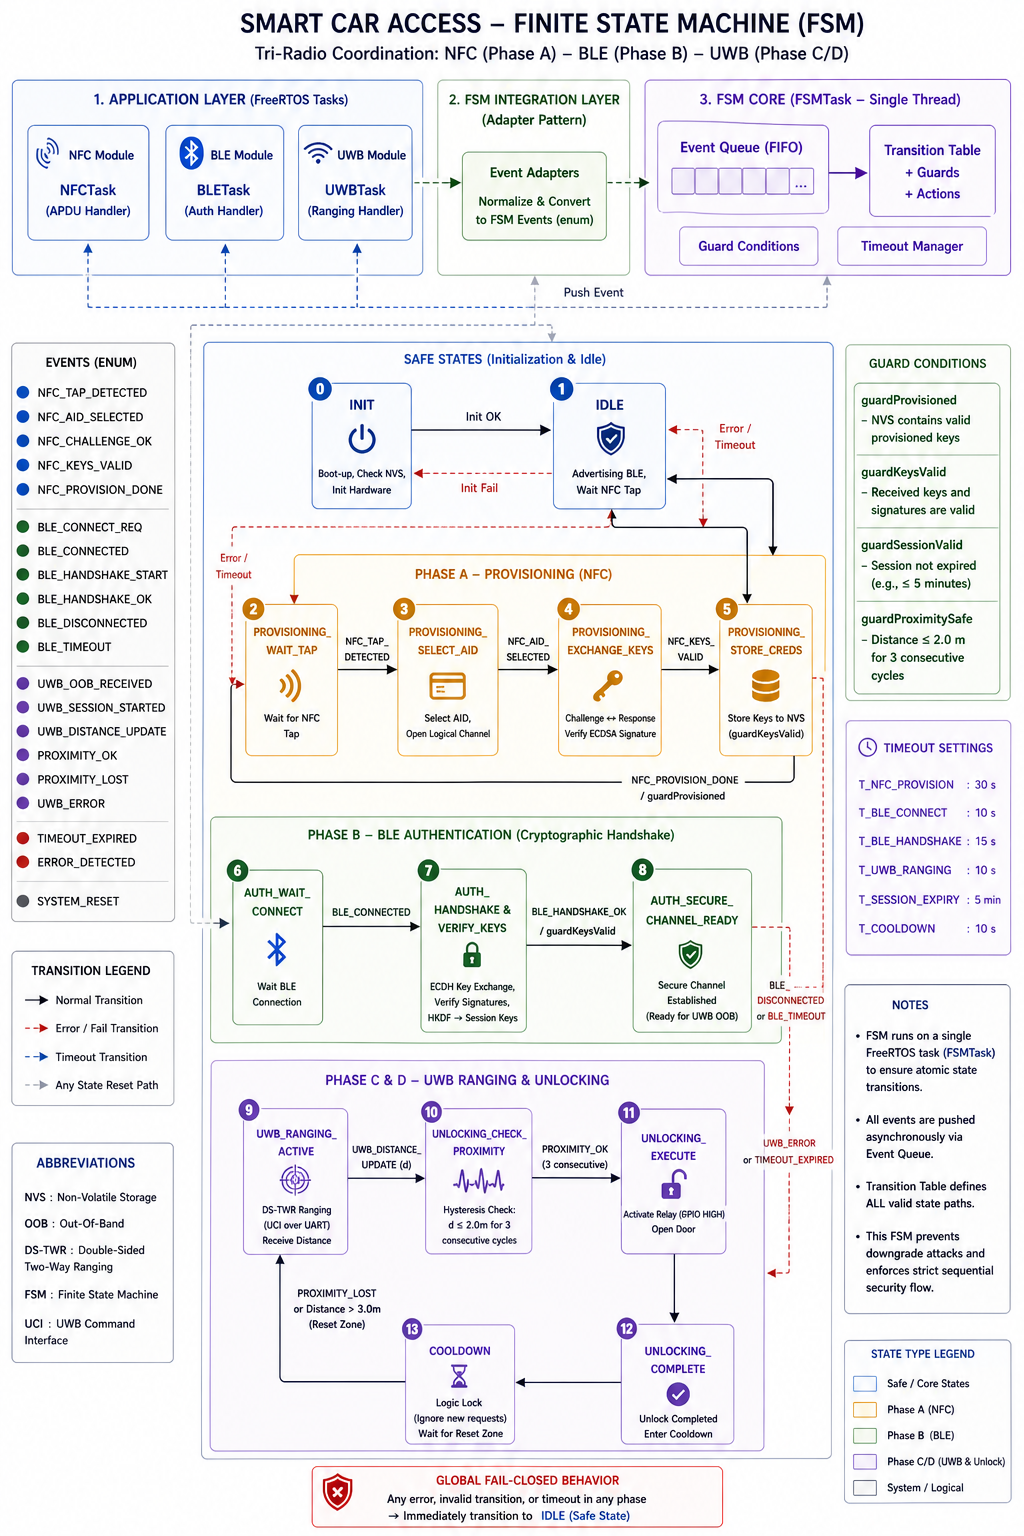
\includegraphics[width=0.9\textwidth]{image/section4/FSMnew.png} 
    \caption{Sơ đồ Máy Trạng thái Xuyên tầng (Cross-layer FSM)}
    \label{fig:fsm_diagram}
\end{figure}

\subsection{Cấu trúc phân lớp FSM}
Kiến trúc FSM trên ESP32 được triển khai dựa trên cơ chế đa luồng (Multi-tasking) của FreeRTOS, bao gồm ba tầng chính:

\begin{enumerate}
  \item \textbf{Tầng Ứng dụng (Application Layer)}: 
  Chạy độc lập trên các FreeRTOS Task tương ứng (\texttt{NFCTask}, \texttt{BLETask}, \texttt{UWBTask}). Tầng này thu thập dữ liệu thô từ các module phần cứng nhưng không có quyền tự thay đổi trạng thái của hệ thống.
  
  \item \textbf{Tầng Tích hợp (FSM Integration Layer)}: 
  Sử dụng Adapter Pattern để chuẩn hóa các sự kiện (Events) riêng lẻ thành dạng enum chung cho FSM (ví dụ: chuyển tín hiệu ngắt từ vi mạch DW3000 thành sự kiện \texttt{UWB\_OOB\_RECEIVED}).
  
  \item \textbf{Tầng Cốt lõi (FSM Core)}: 
  Hoạt động trên một FreeRTOS Task duy nhất (\texttt{FSMTask}) để tránh xung đột tài nguyên, bao gồm:
  \begin{itemize}
    \item \textbf{Hàng đợi sự kiện (Event Queue):} Xử lý bất đồng bộ, giúp FSM không bị treo khi nhận nhiều tín hiệu cùng lúc.
    \item \textbf{Bảng chuyển trạng thái (Transition Table):} Ma trận tĩnh định nghĩa mọi đường dẫn trạng thái hợp lệ.
    \item \textbf{Điều kiện bảo vệ (Guard Conditions):} Xác minh bối cảnh (Context) trước khi cho phép chuyển trạng thái (ví dụ: \texttt{guardKeysValid} hoặc \texttt{guardProvisioned}).
    \item \textbf{Cơ chế Timeout:} Tự động đặt lại trạng thái về \texttt{IDLE} nếu quá trình xác thực không hoàn tất trong thời gian quy định.
  \end{itemize}
\end{enumerate}

\subsection{Phân loại các chuỗi trạng thái}

Các trạng thái được phân định rạch ròi theo 4 giai đoạn bảo mật của hệ thống:

\subsubsection{Trạng thái Khởi tạo và An toàn}
\begin{itemize}
  \item \textbf{INIT}: Trạng thái thiết lập ban đầu (Boot-up). Kiểm tra tính toàn vẹn của CCC Mailbox trong bộ nhớ NVS và khởi động các phần cứng vô tuyến.
  \item \textbf{IDLE}: Trạng thái nghỉ an toàn. Hệ thống duy trì quảng bá BLE và chờ quét thẻ NFC. Mọi lỗi bảo mật hoặc Timeout ở các pha sau đều đưa hệ thống về trạng thái này.
\end{itemize}

\subsubsection{Nhóm trạng thái Phase A - Cấp quyền vật lý}
Chuỗi trạng thái xử lý giao tiếp APDU qua NFC giữa ESP32 và điện thoại (Host Card Emulation):
\begin{itemize}
  \item \textbf{PROVISIONING\_WAIT\_TAP}: Trạng thái Polling, chờ người dùng đưa điện thoại chạm vào đầu đọc NFC.
  \item \textbf{PROVISIONING\_SELECT\_AID}: Thiết lập kết nối logic đến đúng ứng dụng cấp quyền.
  \item \textbf{PROVISIONING\_EXCHANGE\_KEYS}: ESP32 gửi thông điệp thử thách (Challenge), nhận và xác thực chữ ký ECDSA từ điện thoại.
  \item \textbf{PROVISIONING\_STORE\_CREDS}: Chỉ ghi dữ liệu khóa vào NVS khi điều kiện bảo vệ \texttt{guardKeysValid} trả về đúng.
\end{itemize}

\subsubsection{Nhóm trạng thái Phase B - Xác thực kênh truyền}
Quản lý quá trình bắt tay mật mã (Cryptographic Handshake) tầm xa:
\begin{itemize}
  \item \textbf{AUTH\_WAIT\_AUTH0 / AUTH\_WAIT\_CONNECT}: Chờ điện thoại gửi yêu cầu kết nối sau khi đã qua bước kiểm tra \texttt{guardProvisioned}.
  \item \textbf{AUTH\_HANDSHAKE \& VERIFY\_KEYS}: Trạng thái tính toán chuyên sâu (chạy trên \texttt{AuthWorker} task). Thực hiện ECDH Key Exchange và băm HKDF để sinh Session Keys.
  \item \textbf{AUTH\_SECURE\_CHANNEL\_READY}: Kênh BLE bảo mật đã thiết lập. Ở trạng thái này, hệ thống sẵn sàng nhận tải trọng cấu hình UWB (OOB Payload), nhưng \textbf{chưa được phép} bật rơ-le mở cửa.
\end{itemize}

\subsubsection{Nhóm trạng thái C\&D - Đo khoảng cách và Kích hoạt relay}
Tiếp quản phiên làm việc từ Phase B để quyết định mở khóa:
\begin{itemize}
  \item \textbf{UWB\_RANGING\_ACTIVE}: Kích hoạt sau khi nhận được sự kiện \texttt{UWB\_OOB\_RECEIVED}. ESP32 liên tục giao tiếp chuẩn UCI với chip DW3000 để đo khoảng cách theo giao thức DS-TWR.
  \item \textbf{UNLOCKING\_CHECK\_PROXIMITY}: Module \texttt{UwbDoorUnlock} thực hiện kiểm tra Hysteresis. Nếu dữ liệu khoảng cách UWB thỏa mãn điều kiện an toàn (ví dụ: $< 2.0$m trong 3 chu kỳ liên tiếp), kích hoạt sự kiện \texttt{PROXIMITY\_OK}.
  \item \textbf{UNLOCKING\_EXECUTE \& COMPLETE}: FSM gọi hàm cấp điện áp High cho chân GPIO điều khiển Rơ-le cửa, sau đó ghi nhận hoàn tất và đưa hệ thống vào trạng thái \textit{Cooldown} (khóa logic tạm thời).
\end{itemize}